\documentclass{article}

\usepackage{polyglossia}
\usepackage{xcolor}
\usepackage{fontspec}
\usepackage{mathtools}
\usepackage{graphicx}
\setdefaultlanguage{french}
\setlength{\parskip}{4pt}
\newtheorem{definition}{Définition}

\begin{document}

\section{Introduction}

\emph{Qu'est ce qu'un programme ?}

C'est une suite d'instructions.
On utilise souvent la méthapore de la recette de cuisine,
avec ses ingrédients (=données) et les étapes (=instructions).

Voici différents paradigmes de programmation (=manière d'approcher la programmation et de concevoir
les solutions aux problèmes donnés) :

\begin{tabular}{|c|c|c|}
	\hline
	Langages classiques & Langages fonctionnels & Langages logiques \\
	(procéduraux) & & \\
	\hline
	C, Pascal, & LISP, CAML, & PROLOG \\
	FORTRAN, COBOL & Lambda-calculs & \\
	\hline
\end{tabular}

\subsection{Autre paradigme : les langages objets}

\begin{itemize}
	\item \emph{SIMULA} (65-70) : \textbf{Les classes}
		\begin{itemize}
			\item \underline{Principe 1} : on raccroche à la structure de données (champs), 
				les codes qui peuvent les manipuler (méthodes)
		\end{itemize}
	\item \emph{SMALLTALK} (70-75) : \textbf{L'héritage}
		\begin{itemize}
			\item A. Kay (souris, interfaces graphiques)
			\item \underline{Principe 2} : on hiérarchise les classes
		\end{itemize}
	\item En dehors des labos :
		\begin{itemize}
			\item 80 : SMALLTALK
			\item EIFFEL, LISPOBJECT, PASCALOBJECT, C++, JAVA 
		\end{itemize}
\end{itemize}

\subsection{Langages compilés vs interprétés}

\begin{itemize}
	\item Un compilateur traduit un programme (=source) en un fichier exécutable
		par le processeur (généralement en langage assembleur).
	\item Un interpréteur traduit et exécute ligne par ligne.
	\item Ainsi, un interpréteur gagne en souplesse 
		(il peut éviter une ligne qui provoque une erreur), 
		mais perd en rapidité (par exemple, dans une boucle, 
		où il re-traduit les lignes à chaque tour). 
\end{itemize}



\section{Principe de la programmation objet}

Les différences avec la programmation classique :

\begin{itemize}
	\item \textbf{La programmation classique :}
		\begin{itemize}
			\item Les procédures agissent sur les données
				\begin{enumerate}
					\item on a une première idée des procédures
					\item on définit les variables (données)
					\item on écrit les procédures
				\end{enumerate}
			\item une exécution = appels aux procédures dans un ordre,
				en donnant les données nécessaires
		\end{itemize}
	\item \textbf{POO :}
		\begin{itemize}
			\item On pense concept
			\item Programmer : on raccroche à la structure de données (champs), 
				les codes qui peuvent les manipuler (méthodes)
			\item Exécuter : une seule entité homogène : l'objet 
				(aspect données et activations) 
		\end{itemize}
\end{itemize}

\subsection{Les concepts de base}

La modélisation amène à concevoir mes classes (codes et données), 
les objets sont activités par envois de messages lors l'exécution. 

\subsubsection{Classes et instances}

\begin{definition}
	Une classe est un moule (ou matrice) à partir duquel sont générés 
	les objets.

	Un objet généré à partir d'une classe C est une 
	instance de C.

	Une classe a un nom (le nom du concept); elle est constituée d'un 
	ensemble de champs (attributs, variables d'instances) qui décrivent 
	la structure des objets, et d'opérations, appelées méthodes,
	qui leur sont applicables. 
\end{definition}

\textbf{En LOLO} (\sim SMALLTALK)

\begin{verbatim}
classe Compte
	champs credit : Nbe
		   debit : Nbe
FinCompte
\end{verbatim}

\textbf{En JAVA} 

\begin{verbatim}
class Compte {
	int credit;
	int debit;
}
\end{verbatim}

Création d'un objet :
\begin{itemize}
	\item Un objet est créé par appel à un constructeur (new) appliqué à sa 
		classe. Le résultat de la création est un objet qui peut être placé 
		dans une variable, un pointeur sur l'objet.
	 \item Rappel : l'objet créé est dit \emph{instance} de la classe qui
		 l'a créé.
\end{itemize}

\textbf{En LOLO}

\begin{verbatim}
C <- Compte<=new()
\end{verbatim}

\textbf{En JAVA} 

\begin{verbatim}
Compte C = new Compte();
\end{verbatim}

\subsubsection{Méthodes et envois de messages}

\begin{itemize}
	\item La partie dynamique des objets est assurée par l'envoi 
		de messages
	\item Instruction à un objet : Envoyer un message à un objet 
		c'est lui dire le comportement qu'il doit adopter, 
		c'est à dire la méthode qu'il doit s'appliquer.
\end{itemize}

\begin{definition}
	Une méthode est une description, au niveau d'une classe, 
	d'un ensemble d'instructions.

	La méthode contient une liste de paramètres formels; 
	elle peut s'appliquer aux objets instances de la classe.

	Un message est contitué du nom de la méthode (m) et d'une liste 
	de paramètres effectifs.
\end{definition}

\begin{itemize}
	\item Lorsqu'un objet O reçoit un message M, il s’applique 
		la méthode donnée dans M; celle-ci étant définie dans 
		la classe C de l'objet O
\end{itemize}

\textbf{En UML (Langage de Modélisation Unifié)}

\begin{tabular}{|c|}
	\hline
	Nomclasse \\
	\hline
	Champs \\
	\dots \\
	\hline
	Méthodes \\
	\dots \\
	\hline
\end{tabular}

On appelle cela un diagramme de classe.


\textbf{En LOLO}

\begin{verbatim}
Classe Compte
	Champs ...
		   ... 
	Methode deposer(V : Nbre)
		credit <- credit + V
	Methode retirer(V : Nbre)
		credit <- credit - V
	Methode VoirSolde : Nbre
		Return credit - debit
FinCompte

Dupont <- Compte<=new()
Dupont<=deposer(50)
Dupont<=AvoirSolde()
\end{verbatim}

\textbf{En JAVA} 

\begin{verbatim}
Class Compte {
int ...;
...
public void deposer(int V){credit += V;}
public void retirer(int V){credit -= V;}
public int AvoirSolde(){return cerdit - debit}
}

compte Dupont = new Compte();
Dupont.deposer(100);
\end{verbatim}

\subsubsection{L'héritage}

\begin{itemize}
	\item Méthode :
		\begin{enumerate}
			\item Lors de la conception, on regroupe dans une classe commune les
				caractéristiques (ou membres), c’est à dire les champs et méthodes,
				communes de classes se ressemblant
			\item On hiérarchise les classes avec le lien 
				\textcolor{red}{\textbf{« est-une-sorte-de »}}
		\end{enumerate}
\end{itemize}

\begin{definition}
	Une sous classe SC d'une classe C, est une classe sorte de C.

	SC possède par défaut les caractéristiques de C.

	On dit que SC est une spécialisation de C, et que C est une
	généralisation de SC.
\end{definition}

\begin{itemize}
	\item La hiérarchie permet ainsi de factoriser l'écriture (et MAJ=Mise A Jour) 
		de caractéristiques de plusieurs (sous) classes.
	\item On dit qu'une classe (ou objet) hérite des caractéristiques 
		de ses sur-classes.
\end{itemize}

\subsection{L'interprétation des messages}
L’effet d’un message dépend du receveur (l'objet) et de
l'héritage (hiérarchie).

\subsubsection{L'effet dépend du receveur}
\begin{itemize}
	\item Un objet ne peut recevoir un message que si le sélecteur
appartient à la classe de l'objet ou à une de ses sur-classes
	\item  Il est possible d'envoyer deux messages avec le même sélecteur
à deux objets différents qui ne sont pas de la même classe.
Chaque classe implémentant sa propre méthode
\end{itemize}

\subsubsection{L'effet dépend de la hiérarchie d'héritage}
\begin{itemize}
	\item Règle: Lorsqu'un objet reçoit un message de sélecteur M, il recherche
d'abord la méthode de nom M dans sa classe, puis s'il ne la
trouve pas, il recherche en remontant dans la hiérarchie des
classes héritées.
\end{itemize}

\subsubsection{La composition des messages}
\begin{definition}
Lorsqu’un message envoyé à un objet retourne un objet qui lui
même reçoit un message, on dit qu’il y a composition de
messages.
\end{definition}

\subsubsection{Les messages à soi-même}
\begin{itemize}
	\item Les objets ont besoin de s'envoyer des messages à
eux-même
	\item  Il existe une « variable » pour cela appelée (\emph{self} en SMALLTALK
		, \emph{this} en JAVA et C++)
\end{itemize}

\subsubsection{Les méthodes quasi-génériques}
\begin{itemize}
	\item Grâce a l'héritage et self (this)
	\item On peut définir des méthodes attachées à une classe
indépendantes de leurs réalisations dans des sous-classes
\end{itemize}

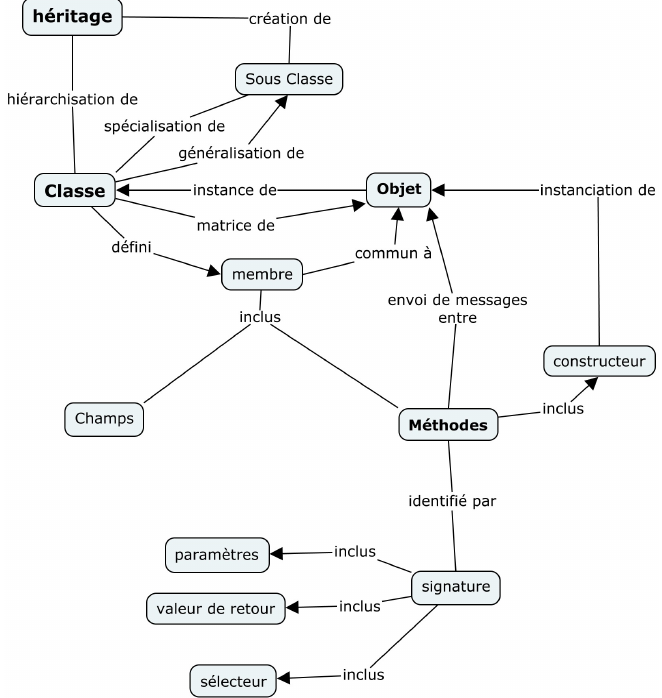
\includegraphics[scale=0.6]{resume}
\centering

\end{document}
